\documentclass{beamer}

\uselanguage{english}
\languagepath{english}
%\deftranslation[to=italian]{Theorem}{Teorema}
%\deftranslation[to=italian]{Definition}{Definizione}
%\deftranslation[to=italian]{Corollary}{Corollario}

\usetheme[progressbar=frametitle, block=fill]{metropolis} % Use metropolis theme

\usepackage[utf8]{inputenc}
\usepackage{forest}
\usepackage{xspace}
\usepackage{xcolor}
\usepackage[normalem]{ulem}
\usepackage[scale=2]{ccicons}  % per le icone creative commons

\usepackage{tikz-cd}
\usepackage{tikz}
\usetikzlibrary{calc} 
\usetikzlibrary{decorations.text}
\usetikzlibrary{decorations.pathreplacing}
\usetikzlibrary{arrows}

%%% inizio comandi per stile per teoremi: "numero. Titolo" %%%
\newtheoremstyle{num.custom-title}
  {\topsep}   % ABOVESPACE
  {\topsep}   % BELOWSPACE
  {\itshape}  % BODYFONT
  {0pt}       % INDENT (empty value is the same as 0pt)
  {\bfseries} % HEADFONT
  {}         % HEADPUNCT
  {5pt plus 1pt minus 1pt} % HEADSPACE
  {\thmnumber{#2.}\thmnote{ #3}}
  
\theoremstyle{num.custom-title}  
\newtheorem{teo_custom-title}[theorem]{} % per usarlo basta \begin{teo_custom-title}[<Titolo teorema>] (usa automaticamente la numerazione di [teo])
%%% fine comandi per stile per teoremi: "numero. Titolo" %%%

%%% inizio comandi per stile per teoremi: "Titolo" %%%
\newtheoremstyle{custom-title}{}{}{\normalfont}{}{\bfseries}{.}{.5em}{\thmnote{#3}#1}
\theoremstyle{custom-title}
\newtheorem*{teo_custom-title_nonum}{}
%%% fine comandi per stile per teoremi: "numero. Titolo" %%%

\newenvironment{claim}[1]{\par\noindent\underline{Claim#1:}\space}{} %per i claim
\newenvironment{claimproof}[1]{\par\noindent\underline{Proof:}\space#1}{\leavevmode\unskip\penalty9999 \hbox{}\nobreak\hfill\quad\hbox{$\blacksquare$}} %per le dimostrazioni dei claim

\DeclareMathOperator{\dom}{dom}
\DeclareMathOperator{\ran}{ran}
\DeclareMathOperator{\orb}{orb}
\DeclareMathOperator{\id}{id}
\DeclareMathOperator{\rk}{rk}
\DeclareMathOperator{\tor}{tor}
\let\o\relax % elimina \o dai comandi già definiti
\DeclareMathOperator{\o}{\mathsf{o}}
\let\Im\relax % elimina \o dai comandi già definiti
\DeclareMathOperator{\Im}{Im}
\DeclareMathOperator{\Zdv}{Zdv}
\DeclareMathOperator{\Hom}{Hom}
\DeclareMathOperator{\End}{End}
\DeclareMathOperator{\Ann}{Ann}
\DeclareMathOperator{\E}{\mathbb{E}}
\DeclareMathOperator{\PP}{\mathcal{P}}
\DeclareMathOperator{\LL}{\mathcal{L}}
\DeclareMathOperator{\Hrtg}{\text{Hrtg}}
\DeclareMathOperator{\J}{\mathcal{J}}
\DeclareMathOperator{\Z}{\mathbb{Z}}
\DeclareMathOperator{\U}{\mathfrak{U}}
\DeclareMathOperator{\PPP}{\mathbb{P}}
\DeclareMathOperator{\V}{\mathcal{V}}
\DeclareMathOperator{\Var}{Var}
\DeclareMathOperator{\Cov}{Cov}
\DeclareMathOperator{\a01}{\{0,1\}^{\star}}
\DeclareMathOperator{\imp}{\Rightarrow}
\DeclareMathOperator{\pmi}{\Leftarrow}
\DeclareMathOperator{\Pic}{Pic}
\DeclareMathOperator{\sm}{\setminus}
\DeclareMathOperator{\sse}{\subseteq}
\DeclareMathOperator{\cl}{cl}
\DeclareMathOperator{\Spec}{Spec}
\DeclareMathOperator{\Tr}{Tr}
\DeclareMathOperator{\spn}{span}
\DeclareMathOperator{\q}{\mathsf{q}}
\DeclareMathOperator{\h}{h}
\DeclareMathOperator{\GL}{GL}
\DeclareMathOperator{\type}{type}
\DeclareMathOperator{\height}{height}
\DeclareMathOperator{\length}{length}
\DeclareMathOperator{\restr}{\upharpoonright}
\DeclareMathOperator{\down}{\downarrow}
\DeclareMathOperator{\up}{\uparrow}
\DeclareMathOperator{\cf}{cf}
\DeclareMathOperator{\mos}{mos}
\DeclareMathOperator{\trcl}{trcl}
\DeclareMathOperator{\Fn}{Fn}
%\DeclareMathOperator{\conc}{^\frown}
%\DeclareMathOperator{\gcd}{GCD}


\newcommand{\AC}{\ensuremath{\mathsf{AC}}\xspace}
\newcommand{\CC}{\ensuremath{\mathsf{CC}}\xspace}
\newcommand{\DC}{\ensuremath{\mathsf{DC}}\xspace}
\newcommand{\ZF}{\ensuremath{\mathsf{ZF}}\xspace}
\newcommand{\ZFC}{\ensuremath{\mathsf{ZFC}}\xspace}
\newcommand{\LS}{\ensuremath{\mathsf{LS}}\xspace}
\newcommand{\AMC}{\ensuremath{\mathsf{AMC}}\xspace}
\newcommand{\TP}{\ensuremath{\mathsf{TP}}\xspace}
\newcommand{\GCH}{\ensuremath{\mathsf{GCH}}\xspace}
\newcommand{\CH}{\ensuremath{\mathsf{CH}}\xspace}
\newcommand{\SH}{\ensuremath{\mathsf{SH}}\xspace}
\newcommand{\nSH}{\ensuremath{\neg\mathsf{SH}}\xspace}
\newcommand{\MA}{\ensuremath{\mathsf{MA}}\xspace}
\newcommand{\ST}{\ensuremath{\mathsf{ST}}\xspace}
\newcommand{\KT}{\ensuremath{\mathsf{KT}}\xspace}
\newcommand{\KH}{\ensuremath{\mathsf{KH}}\xspace}
\newcommand{\FST}{\ensuremath{\mathsf{FST}}\xspace}
\newcommand{\CST}{\ensuremath{\mathsf{CST}}\xspace}
\newcommand{\HRule}{\rule{\linewidth}{0.5mm}} %per la prima pagina
\newcommand{\qedblack}{\hfill $\blacksquare$}
\newcommand{\ol}{\overline}
\newcommand{\ul}{\underline}
\newcommand{\A}{\mathcal{A}}
\newcommand{\B}{\mathcal{B}}
\newcommand{\C}{\mathbb{C}}
\newcommand{\F}{\mathcal{F}}
\newcommand{\I}{\mathcal{I}}
\newcommand{\M}{\mathcal{M}}
\newcommand{\Q}{\mathbb{Q}}
\newcommand{\N}{\mathbb{N}}
\newcommand{\R}{\mathbb{R}}
\newcommand{\G}{\mathcal{G}}
\newcommand{\g}{\mathfrak{g}}
\newcommand{\p}{\mathfrak{p}}
\newcommand{\m}{\mathfrak{m}}
\newcommand{\T}{\mathcal{T}}
\newcommand{\X}{\mathbf{X}}
\newcommand{\x}{\mathbf{x}}
\newcommand{\Ord}{\mathrm{Ord}}
%\newcommand{\b}{\mathfrak{b}}
\newcommand{\IFF}{\Longleftrightarrow}
\newcommand{\conc}{^\frown}
\newcommand{\onto}{\xrightarrow{\text{onto}}}
\newcommand{\inj}{\xrightarrow{\text{1-1}}}
\newcommand{\downmapsto}{%
           \mathrel{\raisebox{.1em}{%
							\rotatebox[origin=c]{-90}{$\mapsto$}}}}
\newcommand{\upmapsto}{%
           \mathrel{\raisebox{.08em}{%
							\rotatebox[origin=c]{90}{$\mapsto$}}}}           
\newcommand{\ndivides}{%
  \mathrel{\mkern.5mu % small adjustment
    % superimpose \nmid to \big|
    \ooalign{\hidewidth$\big|$\hidewidth\cr$\nmid$\cr}%
  }%
}
\newcommand*{\defeq}{\mathrel{\rlap{%
                     \raisebox{0.3ex}{$\cdot$}}%
                     \raisebox{-0.3ex}{$\cdot$}}%
                     =}

\renewcommand{\epsilon}{\varepsilon}
\renewcommand{\phi}{\varphi}
\renewcommand{\H}{\mathcal{H}}
\renewcommand{\S}{\mathcal{S}}
\renewcommand{\O}{\mathcal{O}}
\renewcommand{\P}{\mathbb{P}}
\renewcommand{\u}{\mathbf{u}}
\renewcommand{\L}{\mathcal{L}}
\renewcommand{\iff}{\Leftrightarrow}
\newcommand{\forces}{\Vdash}

\renewcommand{\emph}[1]{\textbf{#1}}




\title{Consistency results concerning $\pmb{\omega_1}$-trees}
%\subtitle{Risultati di consistenza per alberi di altezza $\omega_1$}
\author{Andrea Gadotti \hfill Supervisor: Prof.\ Sy Friedman}
\date{7 February 2017 \hfill Co-supervisor: Prof.\ Matteo Viale}
\institute{Università di Torino}
\titlegraphic{\hfill
\includegraphics[height=1.5cm]{logo.png}}



\begin{document}

%%% diminuisce spazi verticali per displaymode %%%
\setlength{\abovedisplayskip}{1pt}
\setlength{\belowdisplayskip}{1pt}
\setlength{\abovedisplayshortskip}{1pt}
\setlength{\belowdisplayshortskip}{1pt}

\maketitle


\begin{frame}{Indice}
\setbeamertemplate{section in toc}[sections numbered]
\tableofcontents[hideallsubsections]
\end{frame}


\section{``Short'' trees}


\begin{frame}{Definitions of tree}
How can we define trees?

\begin{center}
\begin{forest}
 for tree={grow=north}
	[$\bullet$, 
 		[$\bullet$, 
 			[$\bullet$, [$\bullet$][$\bullet$][$\bullet$]]
 			[$\bullet$]
 			[$\bullet$, [$\bullet$][$\bullet$]]
 			[$\bullet$]
 		]
 		[$\bullet$, 
 			[$\bullet$]
 			[$\bullet$, [$\bullet$, [$\bullet$][$\bullet$]]]
 			[$\bullet$]
 		]
 		[$\bullet$, 
 			[$\bullet$]
 			[$\bullet$, 
 				[$\bullet$, [$\bullet$, [$\bullet$][$\bullet$]][$\bullet$]][$\bullet$]
 			]
 		]
	]
\end{forest}
\end{center}
\end{frame}


\begin{frame}{Definitions of tree}


\begin{block}{Definition 1}
A \emph{tree} is a connected (undirected) graph with no cycles, together with a special node, called \emph{root}.
\end{block}

\pause

Definition 1 is easy to understand, but it doesn't work to deal with LARGE trees (in Set Theory).

\pause

\begin{center}
\textit{``When set theorists say large, they \textbf{mean} large.''}
\end{center}
\vspace{-5pt}
\hfill (Scott Aaronson)

\end{frame}


\begin{frame}{Definitions of tree}

We will see three definitions in total:

\begin{itemize}
\item Definition 1. Easy, not general.
\item Definition 2. Quite easy, not general.
\item Definition 3. Less easy, very general.
\end{itemize}

\end{frame}


\begin{frame}{Ordered sets}

\begin{definition}
Let $A$ be a set. A \emph{partial order} ``$<$'' on $A$ is a binary relation between elements of $A$ which is:
\begin{enumerate}[(i)]
\item irreflexive, i.e.\ $x \not< x$;
\item transitive, i.e.\ $x < y$ and $y < z$ imply $x < z$.
\end{enumerate}
\end{definition}

\pause

\begin{exampleblock}{Example}
Let $S$ be the set of all the finite binary strings. Define the relation ``$<$'' as follows:
\begin{center}
$s < t$ if and only if $s$ is shorter than $t$.
\end{center}
Then $<$ is a partial order on $S$. Observe that if two strings have the same length, then they are not comparable.
\end{exampleblock}

\end{frame}


\begin{frame}{Ordered sets}

\begin{alertblock}{Observation}
There are no ``cycles'' in partially ordered sets!
\end{alertblock}

\begin{center}
\begin{tikzpicture}
\def \n {5}
\def \radius {2cm}
\def \margin {8} % margin in angles, depends on the radius
\def \arrayletters{{"a","b","c","d","e"}}

\foreach \s in {1,...,\n}
{
  \node[draw, circle] at ({360/\n * (\s - 1)}:\radius) {\pgfmathparse{\arrayletters[\s - 1]}\pgfmathresult};
  \draw[->, >=latex] ({360/\n * (\s - 1)+\margin}:\radius) 
    arc ({360/\n * (\s - 1)+\margin}:{360/\n * (\s)-\margin}:\radius);
}
\end{tikzpicture}
\end{center}

If $a<e$ and $e<a$, then $a<a$. Impossible!

\end{frame}


\begin{frame}{Ordered sets}

\begin{definition}
A \emph{linear order} (or \emph{total order}) ``$<$'' on a set $A$ is a partial order such that every two elements of $A$ are comparable, i.e.
\begin{center}
for all $x,y \in A$: \quad $x<y$ or $y<x$ or $x=y$.
\end{center}
\end{definition}

\pause

\begin{exampleblock}{Example}
The canonical order on $\N$ and the canonical order on $\R$.
\end{exampleblock}

\end{frame}


\begin{frame}{Trees of height $\pmb{\leq \omega}$}

We can now give the simplified definition of tree.

\pause

\begin{block}{Definition 2}
A \emph{tree} is a partially ordered set $(T,<)$ such that, for each $x \in T$, the set
\begin{center}
$\down x \defeq \{y \in T : y < x\}$
\end{center}
is finite and linearly ordered by $<$.
\end{block}

\end{frame}


\begin{frame}{Trees of height $\pmb{\leq \omega}$}

\vspace{10pt}

\begin{overprint}

\onslide<1>
\begin{center}
\begin{forest}
 for tree={grow=north}
	[$\bullet$, 
 		[$\bullet$, 
 			[$\bullet$, [$\bullet$][$\bullet$][$\bullet$]]
 			[$\bullet$]
 			[$\bullet$, [$\bullet$][$\bullet$]]
 			[$\bullet$]
 		]
 		[$\bullet$, 
 			[$\bullet$]
 			[$\bullet$, [$\bullet$, [$\bullet$][$\bullet$]]]
 			[$\bullet$]
 		]
 		[$\bullet$, 
 			[$\bullet$]
 			[$\bullet$, 
 				[$\bullet$, [$\bullet$, [$\bullet$][$\bullet$]][$\bullet$]][$\bullet$]
 			]
 		]
	]
\end{forest}
\end{center}


\onslide<2>
\begin{center}
\begin{forest}
 for tree={grow=north}
	[$\bullet$, 
 		[$\bullet$, 
 			[$\bullet$, [$\bullet$][$\bullet$][$\bullet$]]
 			[$\bullet$]
 			[$\bullet$, [$\bullet$][$\bullet$]]
 			[$\bullet$]
 		]
 		[$\bullet$, 
 			[$\bullet$]
 			[$\bullet$, [$\bullet$, [$\bullet$][$\bullet$]]]
 			[$\bullet$]
 		]
 		[$\bullet$, 
 			[$\bullet$]
 			[$\bullet$, 
 				[$\bullet$, [$\bullet$, fill=red [$\bullet$][$\bullet$]][$\bullet$]][$\bullet$]
 			]
 		]
	]
\end{forest}
\end{center}
\scalebox{2}{\textcolor{red}{$x$}}


\onslide<3>
\begin{center}
\begin{forest}
 for tree={grow=north}
	[$\bullet$, fill=blue, 
 		[$\bullet$, 
 			[$\bullet$, [$\bullet$][$\bullet$][$\bullet$]]
 			[$\bullet$]
 			[$\bullet$, [$\bullet$][$\bullet$]]
 			[$\bullet$]
 		]
 		[$\bullet$, 
 			[$\bullet$]
 			[$\bullet$, [$\bullet$, [$\bullet$][$\bullet$]]]
 			[$\bullet$]
 		]
 		[$\bullet$, fill=blue, 
 			[$\bullet$]
 			[$\bullet$, fill=blue, 
 				[$\bullet$, fill=blue, [$\bullet$, fill=red [$\bullet$][$\bullet$]][$\bullet$]][$\bullet$]
 			]
 		]
	]
\end{forest}
\end{center}
\scalebox{2}{\textcolor{red}{$x$}, \textcolor{blue}{${\downarrow} \, x$}}

\end{overprint}

\end{frame}


\begin{frame}{Trees of height $\pmb{\leq \omega}$}

How tall can a tree be, according to Definition 2?

Let $T$ be a tree. We can define the \emph{height} of a node in $T$ and the \emph{$n$-th level} of $T$ in the obvious way. Moreover, if the maximum height of every node in $T$ is $n$, then we say that $T$ has height $n+1$. 

\end{frame}


\begin{frame}{Trees of height $\pmb{\leq \omega}$}

\begin{center}
\begin{forest}
 for tree={grow=north}
	[$\bullet$, 
 		[$\bullet$, 
 			[$\bullet$, [$\bullet$][$\bullet$][$\bullet$]]
 			[$\bullet$]
 			[$\bullet$, [$\bullet$][$\bullet$]]
 			[$\bullet$]
 		]
 		[$\bullet$, 
 			[$\bullet$]
 			[$\bullet$, [$\bullet$, [$\bullet$][$\bullet$]]]
 			[$\bullet$]
 		]
 		[$\bullet$, 
 			[$\bullet$]
 			[$\bullet$, 
 				[$\bullet$, [$\bullet$, [$\bullet$][$\bullet$, fill=red]][$\bullet$]][$\bullet$]
 			]
 		]
	]
\end{forest}
\end{center}
\scalebox{1.5}{\textcolor{red}{$x$}} is a highest node, and $\height(x)=5$. So the tree has height $6$.

\end{frame}


\begin{frame}{Trees of height $\pmb{\leq \omega}$}

But the nodes of $T$ could also be arbitrarily large, meaning that their heights are not bounded by any fixed amount. So $T$ has \emph{infinite} height. More precisely, we say that $T$ has height $\N$. Actually, in this situation we prefer to indicate $\N$ by $\omega$. So we say that $T$ has height $\omega$. 

If $T$ has finite height, then we say that $T$ has height ${<\omega}$.

\end{frame}


\begin{frame}{A simple tree of height $\pmb{\omega}$}

\begin{center}
\begin{forest}
 for tree={grow=north}
	[$\bullet$, 
 		[$\bullet$, 
 			[$\bullet$]
 			[$\bullet$, 
 				[$\bullet$, [$\bullet$, [$\bullet$, [,edge=dashed]]]][$\bullet$]
 			]
 		]
 		[$\bullet$, 
 			[$\bullet$]
 			[$\bullet$]
 			[$\bullet$]
 		]
	]
\end{forest}
\end{center}

\end{frame}



\begin{frame}{The tree \FST}

Recall that $\omega$ is just $\N$.

\pause

The set of \emph{finite binary strings} is
\[
2^{< \omega} \defeq \{s \mid s \colon \{0,\dots,n-1\} \to \{0,1\} \text{ for some } n < \omega\}.
\]
\pause
We define the order ``$<$'' on $2^{< \omega}$ by: $s < t$ iff $s$ is a \emph{prefix} of $t$.

\pause

Then we obtain a binary tree \FST (\textit{finite strings tree}).

\vspace{-7pt}

\begin{center}
\begin{forest}
 for tree={grow=north}
	[$\emptyset$, 
 		[1, 
 			[11,
 				[111, 
 					[,edge=dashed][,edge=dashed]
 				]
 				[110,
 					[,edge=dashed][,edge=dashed]
 				]
 			]
 			[10,
 				[101, 
 					[,edge=dashed][,edge=dashed]
 				]
 				[100,
 					[,edge=dashed][,edge=dashed]
 				]
 			]
 		]
 		[0, 
 			[01,
 				[011, 
 					[,edge=dashed][,edge=dashed]
 				]
 				[010,
 					[,edge=dashed][,edge=dashed]
 				]
 			]
 			[00,
 				[001, 
 					[,edge=dashed][,edge=dashed]
 				]
 				[000,
 					[,edge=dashed][,edge=dashed]
 				]
 			]
 		]
 	]
\end{forest}
\end{center}

\end{frame}



%\begin{frame}{Nozioni di base}
%Sia $T$ un albero.
%\begin{itemize}
%\item L'\emph{altezza} di $x \in T$ è l'ordinale $\type(\down x)$.
%\item L'\emph{$\alpha$-esimo livello di $T$} è l'insieme degli elementi di $T$ che hanno altezza $\alpha$.
%\item L'\emph{altezza di $T$} è il più piccolo ordinale $\gamma$ tale che l'altezza di ogni $x \in T$ è $< \gamma$.
%\item Un \emph{ramo} è un sottoinsieme linearmente ordinato massimale di $T$. L'altezza di un ramo si definisce nello stesso modo.
%\item Un ramo è \emph{cofinale in $T$} se ha la stessa altezza di $T$.
%%\item $T|\alpha$ is the subset of $T$ which contains every element of order strictly less than $\alpha$, i.e.\ $T|\alpha \defeq \cup_{\xi < \alpha} U_\xi$. Obviously $T|\alpha$ has height $\alpha$ if $\alpha \leq \height(T)$.
%%\item We say that a tree $(T_2,<_2)$ is an \emph{extension} of $(T_1,<_1)$ if ${<_1} = {<_2} \cap (T_1 \times T_1)$, an \emph{end-extension} if $T_1=T_2|\alpha$ for some $\alpha$.
%\end{itemize}
%\end{frame}


\begin{frame}{Branches}

The ``classical'' definition of branch is: a path from the root to a leaf.

In our new context, the idea is the same, but the formal definition is different.\\
\ 
\begin{definition}
A \emph{branch} in a tree $T$ is a \textit{maximal linearly ordered subset} of $T$. (i.e.\ a subset of $T$ which is linearly ordered and which is not properly contained in any other linearly ordered subset)
\end{definition}

\end{frame}


\begin{frame}{Branches: examples}

\vspace{10pt}

\begin{overprint}

\onslide<1>
\begin{center}
\begin{forest}
 for tree={grow=north}
	[$\bullet$, 
 		[$\bullet$, 
 			[$\bullet$]
 			[$\bullet$, 
 				[$\bullet$, [$\bullet$, [$\bullet$, [,edge=dashed]]]][$\bullet$]
 			]
 		]
 		[$\bullet$, 
 			[$\bullet$]
 			[$\bullet$]
 			[$\bullet$]
 		]
	]
\end{forest}
\end{center}


\onslide<2>
\begin{center}
\begin{forest}
 for tree={grow=north}
	[$\bullet$, fill=red, 
 		[$\bullet$, 
 			[$\bullet$]
 			[$\bullet$, 
 				[$\bullet$, [$\bullet$, [$\bullet$, [,edge=dashed]]]][$\bullet$]
 			]
 		]
 		[$\bullet$, fill=red, 
 			[$\bullet$]
 			[$\bullet$, fill=red]
 			[$\bullet$]
 		]
	]
\end{forest}
\end{center}
\scalebox{1.3}{\textcolor{red}{A branch.}}


\onslide<3>
\begin{center}
\begin{forest}
 for tree={grow=north}
	[$\bullet$, fill=red, 
 		[$\bullet$, fill=red, 
 			[$\bullet$, fill=red]
 			[$\bullet$, 
 				[$\bullet$, [$\bullet$, [$\bullet$, [,edge=dashed]]]][$\bullet$]
 			]
 		]
 		[$\bullet$
 			[$\bullet$]
 			[$\bullet$]
 			[$\bullet$]
 		]
	]
\end{forest}
\end{center}
\scalebox{1.3}{\textcolor{red}{Another branch.}}


\onslide<4>
\begin{center}
\begin{forest}
 for tree={grow=north}
	[$\bullet$, fill=blue, 
 		[$\bullet$, fill=blue,
 			[$\bullet$]
 			[$\bullet$, fill=blue, 
 				[$\bullet$, fill=blue, [$\bullet$, [$\bullet$, [,edge=dashed]]]][$\bullet$, fill=blue]
 			]
 		]
 		[$\bullet$
 			[$\bullet$]
 			[$\bullet$]
 			[$\bullet$]
 		]
	]
\end{forest}
\end{center}
\scalebox{1.3}{\textcolor{blue}{Not a branch (not linearly ordered).}}


\onslide<5>
\begin{center}
\begin{forest}
 for tree={grow=north}
	[$\bullet$, fill=blue, 
 		[$\bullet$, fill=blue,
 			[$\bullet$]
 			[$\bullet$, fill=blue, 
 				[$\bullet$, [$\bullet$, [$\bullet$, [,edge=dashed]]]][$\bullet$]
 			]
 		]
 		[$\bullet$
 			[$\bullet$]
 			[$\bullet$]
 			[$\bullet$]
 		]
	]
\end{forest}
\end{center}
\scalebox{1.3}{\textcolor{blue}{Not a branch (too small).}}


\onslide<6>
\begin{center}
\begin{forest}
 for tree={grow=north}
	[$\bullet$, fill=red, 
 		[$\bullet$, fill=red,
 			[$\bullet$]
 			[$\bullet$, fill=red, 
 				[$\bullet$, [$\bullet$, [$\bullet$, [,edge=dashed]]]][$\bullet$, fill=red]
 			]
 		]
 		[$\bullet$
 			[$\bullet$]
 			[$\bullet$]
 			[$\bullet$]
 		]
	]
\end{forest}
\end{center}
\scalebox{1.3}{\textcolor{blue}{Not a branch (too small).} Contained in \textcolor{red}{this}}.



\onslide<7>
\begin{center}
\begin{forest}
 for tree={grow=north}
	[$\bullet$, fill=red,
 		[$\bullet$, fill=red,
 			[$\bullet$]
 			[$\bullet$, fill=red,
 				[$\bullet$, fill=red, [$\bullet$, fill=red, [$\bullet$, fill=red, [,edge=dashed]]]][$\bullet$]
 			]
 		]
 		[$\bullet$, 
 			[$\bullet$]
 			[$\bullet$]
 			[$\bullet$]
 		]
	]
\end{forest}
\end{center}
\scalebox{1.3}{\textcolor{blue}{Not a branch (too small).} And also in \textcolor{red}{this}}.

\end{overprint}

\end{frame}


\begin{frame}{Cofinal branches}

It is immediate to define the height of a branch, in the same way we did for trees.

We are interested in ``special'' branches.

\pause

\begin{definition}
A \emph{cofinal} branch of a tree $T$ is a branch which has the same height of $T$.
\end{definition}

\end{frame}


\begin{frame}{Cofinal branches}

In nature, every tree has a ``cofinal'' branch.

\begin{center}
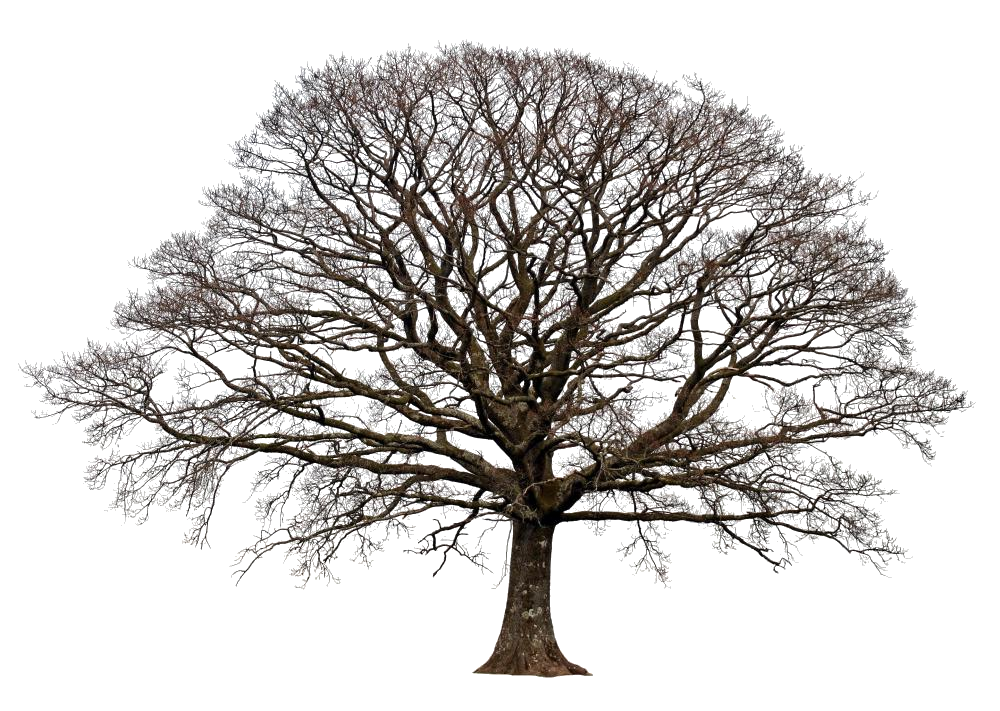
\includegraphics[scale=0.3]{tree_nature.png}
\end{center}

\end{frame}


\begin{frame}{Cofinal branches}

This is clearly true also for trees of finite height. If a tree has height (e.g.)\ $6$, then there is a node of height $5$, i.e.\ a branch of height $6$.

\begin{center}
\begin{forest}
 for tree={grow=north}
	[$\bullet$, fill=red, 
 		[$\bullet$, 
 			[$\bullet$, [$\bullet$][$\bullet$][$\bullet$]]
 			[$\bullet$]
 			[$\bullet$, [$\bullet$][$\bullet$]]
 			[$\bullet$]
 		]
 		[$\bullet$, 
 			[$\bullet$]
 			[$\bullet$, [$\bullet$, [$\bullet$][$\bullet$]]]
 			[$\bullet$]
 		]
 		[$\bullet$, fill=red, 
 			[$\bullet$]
 			[$\bullet$, fill=red, 
 				[$\bullet$, fill=red, [$\bullet$, fill=red [$\bullet$, fill=red][$\bullet$]][$\bullet$]][$\bullet$]
 			]
 		]
	]
\end{forest}
\end{center}

\end{frame}


\begin{frame}{Cofinal branches}

Some trees of height $\omega$ have cofinal branches.

\begin{center}
\begin{forest}
 for tree={grow=north}
	[$\bullet$, fill=red,
 		[$\bullet$, fill=red,
 			[$\bullet$]
 			[$\bullet$, fill=red,
 				[$\bullet$, fill=red, [$\bullet$, fill=red, [$\bullet$, fill=red, [,edge=dashed]]]][$\bullet$]
 			]
 		]
 		[$\bullet$, 
 			[$\bullet$]
 			[$\bullet$]
 			[$\bullet$]
 		]
	]
\end{forest}
\end{center}

\end{frame}


\begin{frame}{Cofinal branches}

Does \textit{every} tree have a cofinal branch?

The answer is: \pause NO.

\pause

\begin{center}
\begin{forest}
 for tree={grow=north}
	[$\bullet$, [,edge=dashed, [,edge=dashed]], [,edge=dashed, [,edge=dashed]], [,edge=dashed, [,edge=dashed]], [,edge=dashed, [,edge=dashed]], [,edge=dashed, [,edge=dashed]], [,edge=dashed, [,edge=dashed]], [,edge=dashed, [,edge=dashed]], [,edge=dashed, [,edge=dashed]], [,edge=dashed, [,edge=dashed]], [,edge=dashed, [,edge=dashed]], [,edge=dashed, [,edge=dashed]],
 		[$\bullet$, 
 			[$\bullet$,
	 			[$\bullet$, 
	 				[$\bullet$,
	 					[$\bullet$,
 						]]]]]
 		[$\bullet$, 
 			[$\bullet$,
	 			[$\bullet$, 
	 				[$\bullet$,
					]]]]
 		[$\bullet$, 
 			[$\bullet$,
	 			[$\bullet$, 
				]]]
 		[$\bullet$, 
 			[$\bullet$,
			]]
 		[$\bullet$, 
		]
	]
\end{forest}
\end{center}

\end{frame}


\begin{frame}{Cofinal branches}

\begin{exampleblock}{Question}
Is there any sufficient condition for a tree of height $\omega$ to have a cofinal branch?
\end{exampleblock}

\end{frame}


\begin{frame}{Back to \FST}
\vspace{5pt}

\begin{overprint}
\onslide<1> In \FST, the height of each node corresponds to its length as string. Hence the $n$-th level contains exactly the strings in \FST of length $n$. 

\onslide<2> So: 
\begin{itemize}
\item[\textcolor{mLightBrown}{$\bullet$}] \FST has height $\omega$;
\item[\textcolor{mLightBrown}{$\bullet$}] the levels of \FST are all finite sets;
\item[\textcolor{mLightBrown}{$\bullet$}] $\{0^n : n < \omega\}$ is a cofinal branch (where $0^n$ means $\overbrace{0000 \ldots}^{n}$).\\
$\{1^n : n < \omega\}$ as well.
\end{itemize}
\end{overprint}

\vspace{-10pt}

\begin{center}
\begin{forest}
 for tree={grow=north}
	[$\emptyset$, 
 		[1, 
 			[11,
 				[111, 
 					[,edge=dashed][,edge=dashed]
 				]
 				[110,
 					[,edge=dashed][,edge=dashed]
 				]
 			]
 			[10,
 				[101, 
 					[,edge=dashed][,edge=dashed]
 				]
 				[100,
 					[,edge=dashed][,edge=dashed]
 				]
 			]
 		]
 		[0, 
 			[01,
 				[011, 
 					[,edge=dashed][,edge=dashed]
 				]
 				[010,
 					[,edge=dashed][,edge=dashed]
 				]
 			]
 			[00,
 				[001, 
 					[,edge=dashed][,edge=dashed]
 				]
 				[000,
 					[,edge=dashed][,edge=dashed]
 				]
 			]
 		]
 	]
\end{forest}
\end{center}

\end{frame}


\begin{frame}{König's lemma}

Last observations about \FST hold in general:

\pause

\begin{lemma}[König, 1927]
Let $T$ be a tree of height $\omega$. If the levels of $T$ are finite sets, then $T$ has a cofinal branch.
\end{lemma}

\pause

\begin{exampleblock}{Question}
Is it possible to generalize König's lemma to cardinals greater than $\omega$?
\end{exampleblock}

\end{frame}


\section{Cardinals}


\begin{frame}{Cardinalities}

Let $A$ be a set. The \emph{cardinality} of $A$ is \textit{the number of elements which belong to $A$}.

But this definition works only for finite sets. For the general case, we say that:

\begin{definition}
Two sets $A$ and $B$ have the same cardinality if and only if there exists a bijection between $A$ and $B$ (i.e.\ a one-to-one correspondence between the elements of $A$ and $B$).
\end{definition}

A set is called \emph{countable} if it has the same cardinality of $\N$. The cardinality of $\N$ is indicated by $\omega$, and it is the \textit{smallest infinite cardinal}. A set $A$ is called \emph{uncountable} if its cardinality is greater than $\omega$ (i.e.\ there exists no function from $\N$ \emph{onto} $A$).\\
Example: $\R$ is uncountable. (\textit{Cantor's diagonal argument})

\end{frame}


\begin{frame}{Cardinalities}

For every cardinal $\kappa$, there is a smallest cardinal greater than $\kappa$. We indicate such cardinal with $\kappa^+$.

So $\omega^+$ is the smallest uncountable cardinal. The cardinal $\omega^+$ is usually called $\omega_1$.

\end{frame}


\section{BIG trees}

\begin{frame}{Well-ordered sets}

To deal with trees of arbitrary height, we first need to generalize Definition 2. In order to do this, we need to define well-ordered sets.

\begin{definition}
A partial order $(P,<)$ is a \emph{well-order} if it is linear and every non-empty subset of $P$ has a minimum.
\end{definition}

\pause

\begin{exampleblock}{Examples}
\begin{itemize}
\item The canonical order on $\N$ is a well-order. 
\item The canonical order on $\Z$ is \textit{not} a well-order.
\item The canonical order on $\R$ is \textit{not} a well-order.
\end{itemize}
\end{exampleblock}

\end{frame}


\begin{frame}{Trees}

\begin{block}{Definition 3}
A \emph{tree} is a partially ordered set $(T,<)$ such that, for each $x \in T$, the set
\begin{center}
$\down x \defeq \{y \in T : y < x\}$
\end{center}
is \sout{finite and linearly ordered} well-ordered by $<$.
\end{block}

\pause

The definitions of level and height of a node/tree/branch can be easily generalized to work also with Definition 3.
\end{frame}


\begin{frame}{Attempt of generalization}

\begin{lemma}[König, 1927]
Let $T$ be a tree of height $\omega$. If the levels of $T$ are finite sets, then $T$ has a cofinal branch.
\end{lemma}

The generalization of König's lemma for $\omega_1$ would be:

\pause

\begin{block}{Conjecture}
\textit{Let $T$ be a tree of height $\omega_1$. If the levels of $T$ are countable sets, then $T$ has a cofinal branch.}
\end{block}

\pause

\begin{exampleblock}{Question}
Is the conjecture true?
\end{exampleblock}

\end{frame}



\begin{frame}{A tree of height $\pmb{\omega_1}$}

\begin{overprint}
\onslide<1> Recall that $\omega_1$ is the smallest cardinal greater than $\omega$.
\onslide<2-3> Recall that $\omega_1$ is the smallest cardinal greater than $\omega$.\\
Consider the tree $(\CST,<)$ of \emph{countable binary strings}, i.e.
\[
\CST \defeq \{s \mid s \colon \alpha \to \{0,1\} \text{ with $\alpha < \omega_1$ and $s$ has finitely-many 1's}\}
\]
and $s<t$ iff $s$ is a prefix of $t$.

%\onslide<3> Consideriamo l'albero $(T,<)$ dove
%\[
%T \defeq \{s \mid s \colon \alpha \to 2 \text{ con $\alpha < \omega_1$ e $s$ ha un numero finito di 1}\}
%\]
%e $<$ è come prima $\subsetneq$. Con $0^\alpha$ indichiamo $\underbrace{00000000 \ldots}_{\alpha}$

\onslide<4>
\vspace{-2pt}
Observe that:
\vspace{-4pt}
\begin{itemize}
\item[\textcolor{mLightBrown}{$\bullet$}] \CST has height $\omega_1$;
\item[\textcolor{mLightBrown}{$\bullet$}] the levels of \CST are all countable; 
\item[\textcolor{mLightBrown}{$\bullet$}] $\{0^\alpha : \alpha {<} \omega_1\}$ is a (cofinal) branch in \CST. $\{1^\alpha : \alpha {<} \omega_1\}$ is \underline{not}.
\end{itemize}
\end{overprint}

\vspace{-18pt}

\visible<3->{
\begin{center}
\begin{forest}
 for tree={grow=north}
	[$\emptyset$, 
 		[1, 
 			[11,
 				[111, 
 					[$\vdots$,edge=dashed [,edge=dashed]]
 				]
 				[110,
 					[$\vdots$,edge=dashed [,edge=dashed]]
 				]
 			]
 			[10,
 				[101, 
 					[$\vdots$,edge=dashed [,edge=dashed]]
 				]
 				[100,
 					[$\vdots$,edge=dashed [,edge=dashed]]
 				]
 			]
 		]
 		[0, 
 			[01,
 				[011, 
 					[$\vdots$,edge=dashed [,edge=dashed]]
 				]
 				[010,
 					[$\vdots$,edge=dashed [,edge=dashed]]
 				]
 			]
 			[00,
 				[001, 
 					[$\vdots$,edge=dashed [,edge=dashed]]
 				]
 				[000,
 					[$0^\alpha$,edge=dashed [,edge=dashed]]
 				]
 			]
 		]
 	]
\end{forest}
\end{center}
}
\end{frame}


\begin{frame}{Aronszajn trees}

\begin{block}{Conjecture}
\textit{Let $T$ be a tree of height $\omega_1$. If the levels of $T$ are countable sets, then $T$ has a cofinal branch.}
\end{block}

\pause

The conjecture is \emph{false}.\\
\ 
\begin{theorem}[Aronszajn, 1934]
There exists an Aronszajn tree, i.e.\ a tree of height $\omega_1$ whose levels are countable, which has no cofinal branch.
\end{theorem}

\end{frame}


\section{Suslin's hypothesis}


\begin{frame}{Antichains}

Let's try to strengthen the assumptions in our conjecture to see if we get at least something...

\begin{definition}
A subset $A$ of a tree is an \emph{antichain} if every two nodes in $A$ are incomparable, i.e. 
\begin{center}
for all $x,y \in A$: \quad $x \nless y$ and $y \nless x$.
\end{center}
\end{definition}

Every level is trivially an antichain.

\end{frame}


\begin{frame}{Antichains}

\vspace{10pt}

\begin{overprint}

\onslide<1>
\begin{center}
\begin{forest}
 for tree={grow=north}
	[$\bullet$, 
 		[$\bullet$, 
 			[$\bullet$, [$\bullet$][$\bullet$][$\bullet$]]
 			[$\bullet$]
 			[$\bullet$, [$\bullet$][$\bullet$]]
 			[$\bullet$]
 		]
 		[$\bullet$, 
 			[$\bullet$]
 			[$\bullet$, [$\bullet$, [$\bullet$][$\bullet$]]]
 			[$\bullet$]
 		]
 		[$\bullet$, 
 			[$\bullet$]
 			[$\bullet$, 
 				[$\bullet$, [$\bullet$, [$\bullet$][$\bullet$]][$\bullet$]][$\bullet$]
 			]
 		]
	]
\end{forest}
\end{center}


\onslide<2>
\begin{center}
\begin{forest}
 for tree={grow=north}
	[$\bullet$, 
 		[$\bullet$, 
 			[$\bullet$, fill=blue, [$\bullet$][$\bullet$][$\bullet$]]
 			[$\bullet$, fill=blue]
 			[$\bullet$, fill=blue, [$\bullet$][$\bullet$]]
 			[$\bullet$, fill=blue]
 		]
 		[$\bullet$, 
 			[$\bullet$, fill=blue]
 			[$\bullet$, fill=blue, [$\bullet$, [$\bullet$][$\bullet$]]]
 			[$\bullet$, fill=blue]
 		]
 		[$\bullet$, 
 			[$\bullet$, fill=blue]
 			[$\bullet$, fill=blue, 
 				[$\bullet$, [$\bullet$, [$\bullet$][$\bullet$]][$\bullet$]][$\bullet$]
 			]
 		]
	]
\end{forest}
\end{center}


\onslide<3>
\begin{center}
\begin{forest}
 for tree={grow=north}
	[$\bullet$, 
 		[$\bullet$, 
 			[$\bullet$, [$\bullet$, fill=blue][$\bullet$][$\bullet$]]
 			[$\bullet$, fill=blue]
 			[$\bullet$, fill=blue, [$\bullet$][$\bullet$]]
 			[$\bullet$, fill=blue]
 		]
 		[$\bullet$, 
 			[$\bullet$]
 			[$\bullet$, [$\bullet$, [$\bullet$, fill=blue][$\bullet$]]]
 			[$\bullet$]
 		]
 		[$\bullet$, 
 			[$\bullet$]
 			[$\bullet$, 
 				[$\bullet$, [$\bullet$, [$\bullet$][$\bullet$, fill=blue]][$\bullet$]][$\bullet$, fill=blue]
 			]
 		]
	]
\end{forest}
\end{center}

\end{overprint}

\end{frame}

\begin{frame}{Suslin trees}

\begin{block}{Conjecture (FALSE)}
\textit{Let $T$ be a tree of height $\omega_1$. If the levels of $T$ are countable sets, then $T$ has a cofinal branch.}
\end{block}

\pause

\begin{block}{Suslin's hypothesis}
\textit{Let $T$ be a tree of height $\omega_1$. If the \sout{levels} antichains of $T$ are countable sets, then $T$ has a cofinal branch.}
\end{block}

\pause

\begin{definition}
A \emph{Suslin tree} is a tree of height $\omega_1$ whose antichains are countable, but which has no cofinal branch.
\end{definition}

\pause

So Suslin's hypothesis is true if and only if there exists \emph{no} Suslin tree.

\end{frame}


\begin{frame}{Suslin trees}

\begin{exampleblock}{Question}
Is there any Suslin tree?
\end{exampleblock}

The answer is: \pause \textit{There is no answer.} \pause And we can prove that there is no answer. \pause

In other words, the existence of Suslin trees is not provable nor refutable in \ZFC, the system of \textit{standard axioms} for mathematics. We say that it is \emph{independent} of \ZFC. More precisely:

\begin{theorem}[Tennenbaum, 1963]
There is a ``universe'' (i.e.\ a model of \ZFC) in which there exists a Suslin tree.
\end{theorem}

\begin{theorem}[Solovay-Tennenbaum, 1971]
There is a ``universe'' (i.e.\ a model of \ZFC) in which there exists no Suslin tree.
\end{theorem}

\end{frame}


\begin{frame}{Forcing}

The proofs of both theorems are based on \emph{forcing}. Forcing is an extremely advanced technique, which can be used to produce universes which satisfy theorems ``at will''.

It was invented by Paul Cohen in 1963 to show the independence of the \emph{Continuum Hypothesis}.

Forcing is still the main tool in Set Theory. It is used and improved by set theorists every day to prove the independence of new statements (many of them about trees).

\end{frame}


\begin{frame}[plain]

\begin{center}
\Large \textbf{Thank you for your attention!}
\end{center}

\vspace{30pt}

Slides and thesis (with \LaTeX\ sources): \url{github.com/korg91}.

\vspace{15pt}

\ccbysa
\end{frame}



\end{document}






























